% !TEX root = ../presentation.tex
% !BIB program = biber
% !TEX program = xelatex

\section[short]{hierarchical vaes know what they don't know}

\begin{frame}
    \frametitle{Results on diverse datasets}
    \begin{columns}
        \begin{column}{0.45\textwidth}
            \hfill
            \begin{table}[t]
                \centering
                \resizebox{0.9\textwidth}{!}{%
                \begin{tabular}{llrrr}
                    \toprule
                    OOD dataset & Metric & AUROC$\uparrow$ & AUPRC$\uparrow$ & FPR80$\downarrow$ \\
                    \midrule
                    \multicolumn{5}{c}{\textbf{Trained on CIFAR10}} \\
                    \midrule
                    SVHN          &  $LLR^{>2}$  &  0.811  &  0.837  &  0.394  \\
                    CIFAR10       &  $LLR^{>1}$  &  0.469  &  0.479  &  0.835  \\
                    \midrule
                    \multicolumn{5}{c}{\textbf{Trained on SVHN}} \\
                    \midrule
                    CIFAR10            &  $LLR^{>1}$       &  $0.939$  &  $0.950$  &  $0.052$  \\
                    SVHN               &  $LLR^{>1}$       &  $0.489$  &  $0.484$  &  $0.799$  \\
                    \bottomrule
                \end{tabular}
                }
            \end{table}
            \hfill
        \end{column}
        \begin{column}{0.55\textwidth}
            \hfill
            \begin{table}[t]
                \centering
                \resizebox{0.9\textwidth}{!}{%
                \begin{tabular}{llrrr}
                    \toprule
                    OOD dataset & Metric & AUROC$\uparrow$ & AUPRC$\uparrow$ & FPR80$\downarrow$ \\
                    \midrule
                    \multicolumn{5}{c}{\textbf{Trained on FashionMNIST}} \\
                    \midrule
                    MNIST                    & $LLR^{>1}$             &  0.986  &  0.987  &  0.011 \\
                    notMNIST                 &  $LLR^{>1}$            &  0.998  &  0.998  &  0.000 \\
                    KMNIST                   &  $LLR^{>1}$            &  0.974  &  0.977  &  0.017 \\
                    Omniglot28x28            &  $LLR^{>2}$            &  1.000  &  1.000  &  0.000 \\
                    Omniglot28x28Inverted    &  $LLR^{>1}$            &  0.954  &  0.954  &  0.050 \\
                    SmallNORB28x28           &  $LLR^{>2}$            &  0.999  &  0.999  &  0.002 \\
                    SmallNORB28x28Inverted   &  $LLR^{>2}$            &  0.941  &  0.946  &  0.069 \\
    {\color{black!60}FashionMNIST}             &  $LLR^{>1}$            &  0.488  &  0.496  &  0.811 \\
                    \midrule
                    \multicolumn{5}{c}{\textbf{Trained on MNIST}} \\
                    \midrule
                    FashionMNIST                   &  $LLR^{>1}$  &  $0.999$  &  $0.999$  &  $0.000$ \\
                    notMNIST                       &  $LLR^{>1}$  &  $1.000$  &  $0.999$  &  $0.000$ \\
                    KMNIST                         &  $LLR^{>1}$  &  $0.999$  &  $0.999$  &  $0.000$ \\
                    Omniglot28x28                  &  $LLR^{>1}$  &  $1.000$  &  $1.000$  &  $0.000$ \\
                    Omniglot28x28Inverted          &  $LLR^{>1}$  &  $0.944$  &  $0.953$  &  $0.057$ \\
                    SmallNORB28x28                 &  $LLR^{>1}$  &  $1.000$  &  $1.000$  &  $0.000$ \\
                    SmallNORB28x28Inverted         &  $LLR^{>1}$  &  $0.985$  &  $0.987$  &  $0.000$ \\
    {\color{black!60}MNIST}                          &  $LLR^{>2}$  &  $0.515$  &  $0.507$  &  $0.792$ \\
                    \bottomrule
                \end{tabular}
                }
            \end{table}
            \hfill
        \end{column}
    \end{columns}
\end{frame}

% ======================================================================================================================

\section{a brief overview of unsupervised speech representation learning}

\begin{frame}
    \frametitle{Types of self-supervised speech representation learning methods}
    
    Schematic of self-supervised methods. Each subfigure illustrates the loss computation for a single time-step. The temporal subscript has been left out for simplicity.

    \begin{figure}
        \centering
        \setlength\tabcolsep{1.5pt}
        \resizebox*{\textheight}{!}{%
        \begin{tabular}{>{\centering\arraybackslash} m{4mm}  >{\centering\arraybackslash} m{0.40\textwidth}|>{\centering\arraybackslash} m{0.40\textwidth}}
            & {\small \textsc{predictive}} & {\small \textsc{masking-based}} \\
            \rotatebox{90}{{\small \textsc{reconstruct}}} & 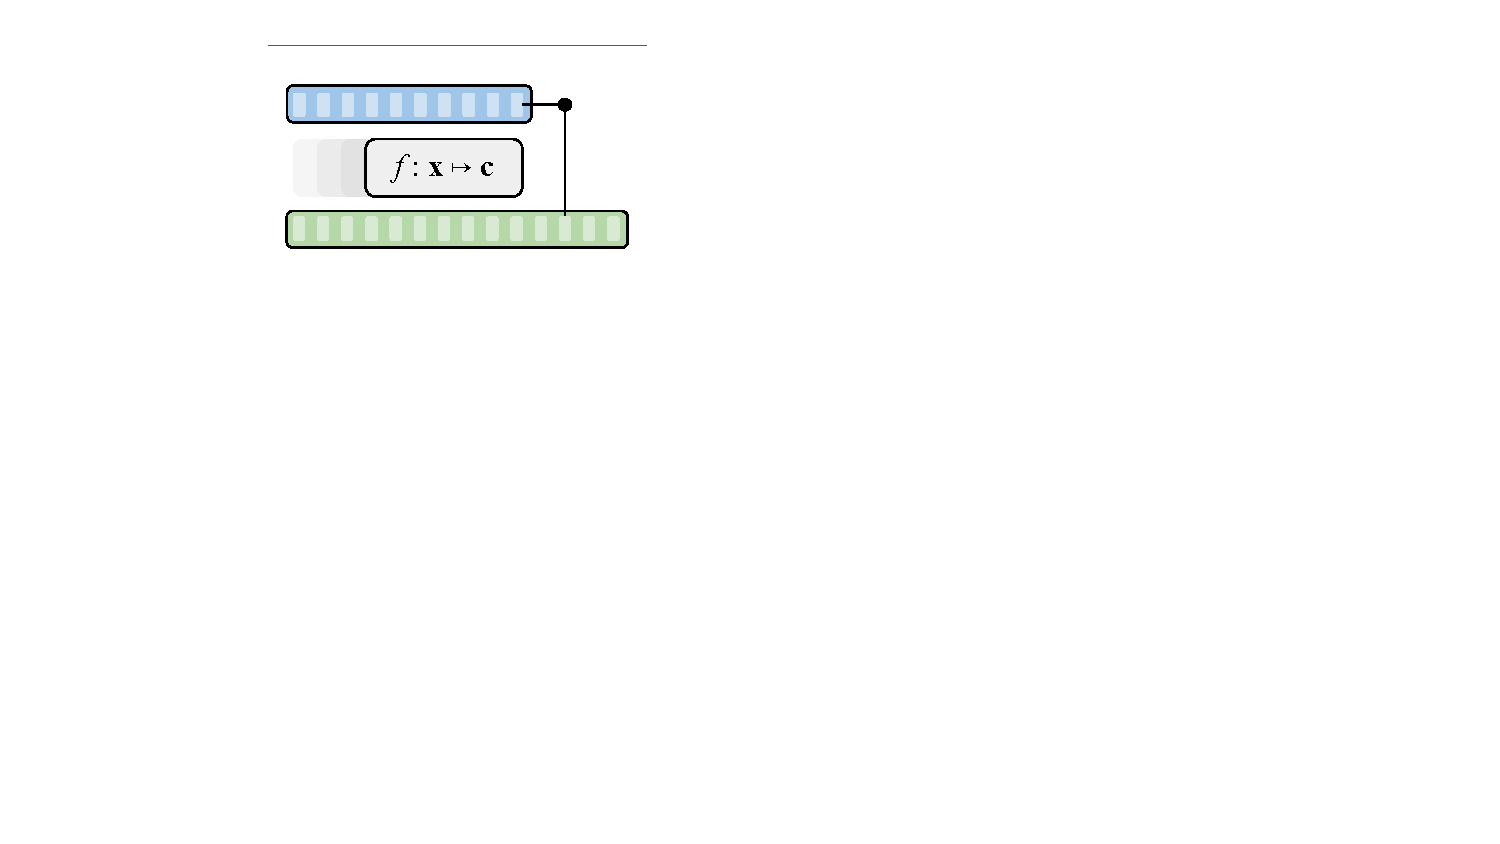
\includegraphics[width=0.40\textwidth]{../graphics/paper_brief/REC_PRD.pdf} & 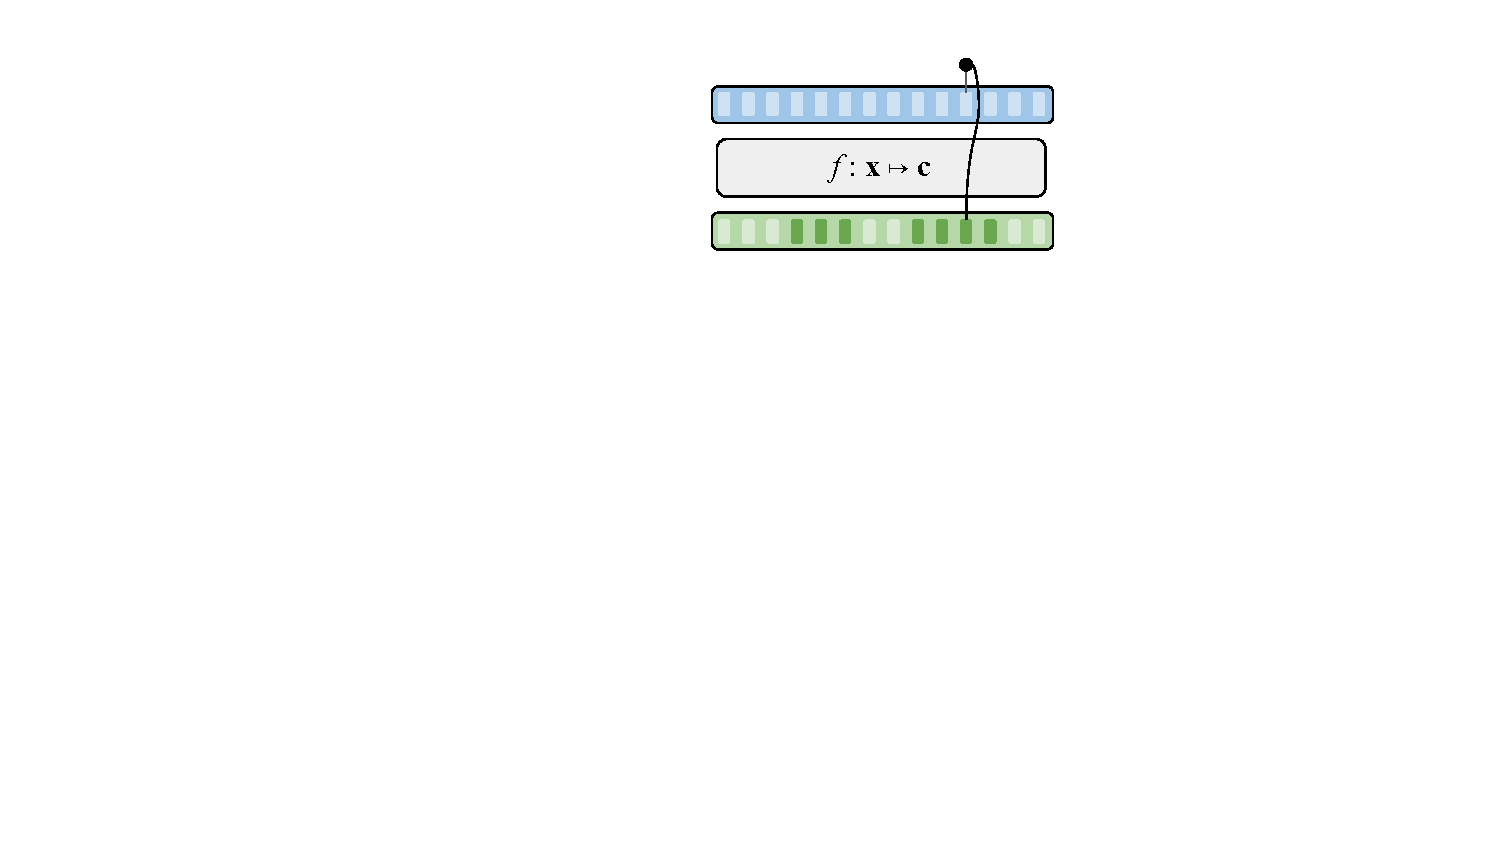
\includegraphics[width=0.40\textwidth]{../graphics/paper_brief/REC_MSK.pdf}  \\
            \midrule
            \rotatebox{90}{{\small \textsc{contrastive}}} & 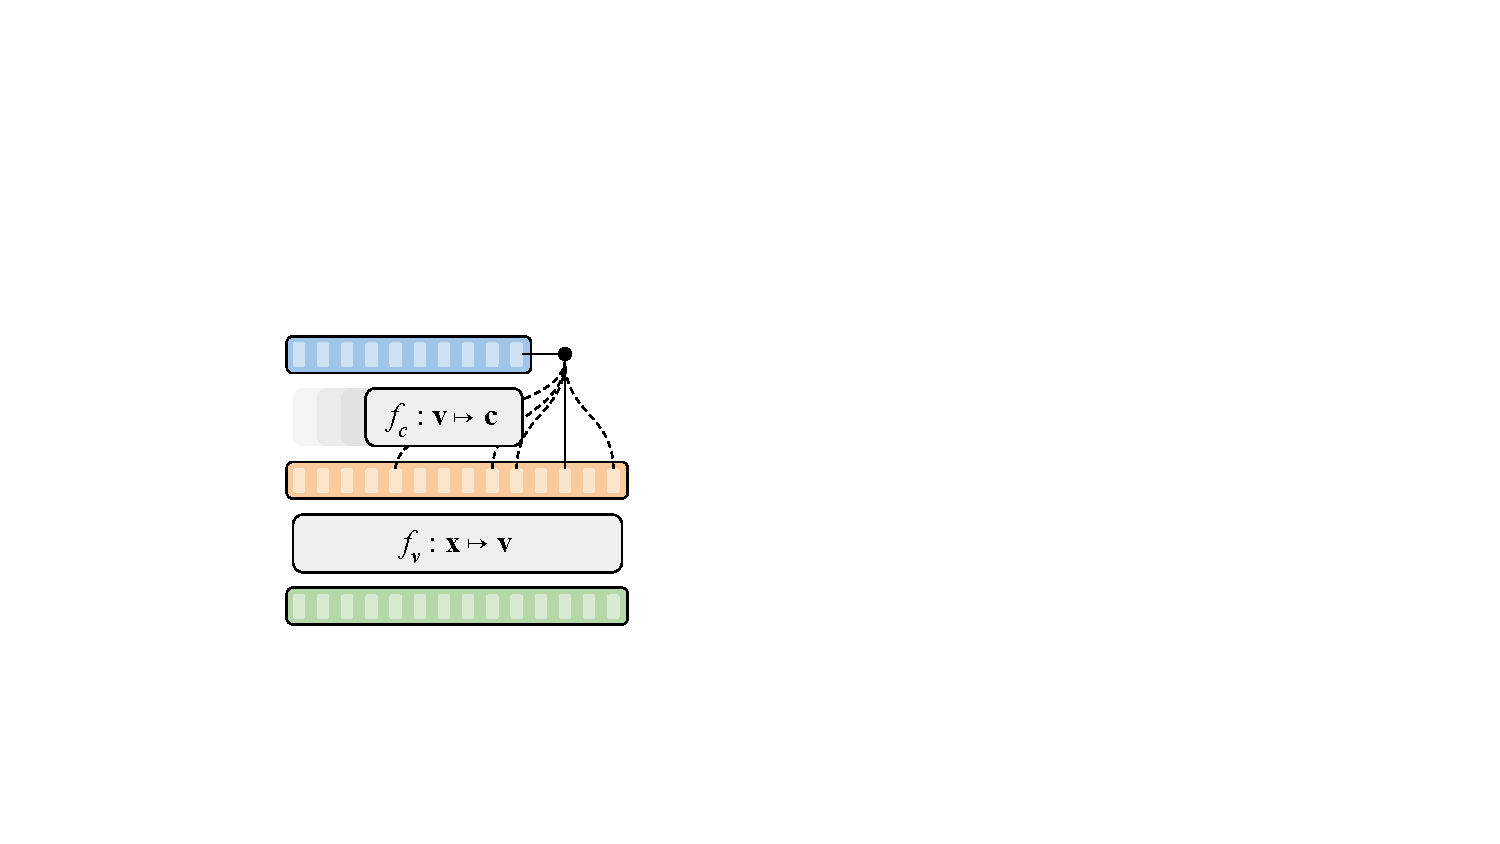
\includegraphics[width=0.40\textwidth]{../graphics/paper_brief/CON_PRD.pdf} & 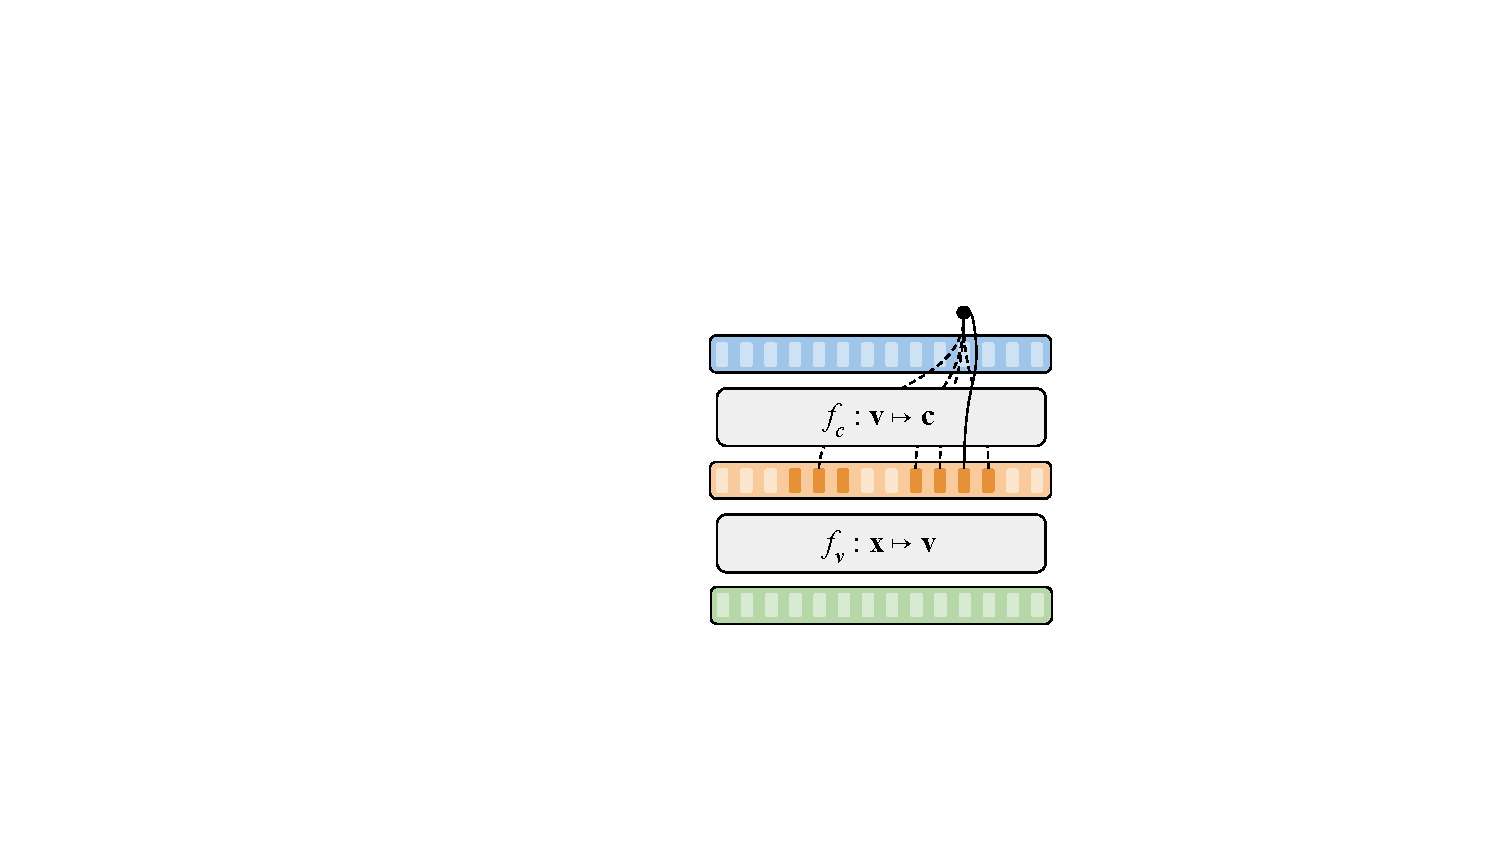
\includegraphics[width=0.40\textwidth]{../graphics/paper_brief/CON_MSK.pdf}
        \end{tabular}
        }
    \end{figure}
\end{frame}


\begin{frame}
    \frametitle{Overview: Representation Learning for Speech}

    \begin{columns}

        \begin{column}{0.4\textwidth}
            \begin{itemize}
                \item We focus on two primary categories:
                \begin{itemize}
                    \item Self-supervised learning (SSL)
                    \item Probabilistic latent variable models (LVMs)
                \end{itemize}
                \item Recent developments have been driven by self-supervised learning.
                \item A model-by-model overview: Focus on speech recognition.
            \end{itemize}
        \end{column}

        \begin{column}{0.6\textwidth}

            \begin{tikzpicture}
                \only<1->{
                    \node[anchor=south west,inner sep=0] (A) at (0,0) {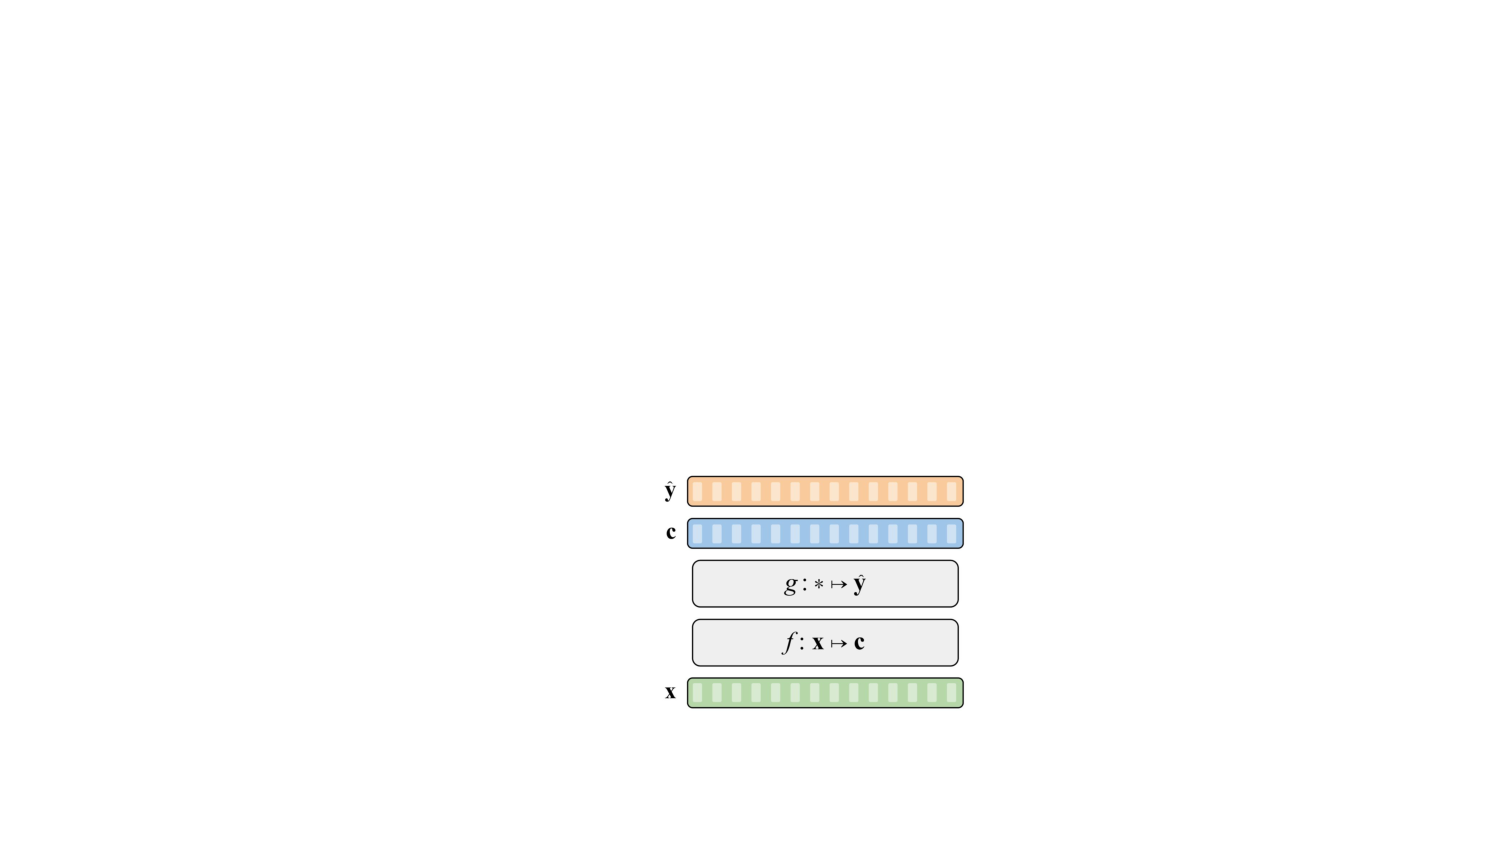
\includegraphics[height=0.4\textheight]{figures/brief-paradigms-ssl.pdf}};
                    \node[anchor=south west,inner sep=0] (B) at (4.2,0) {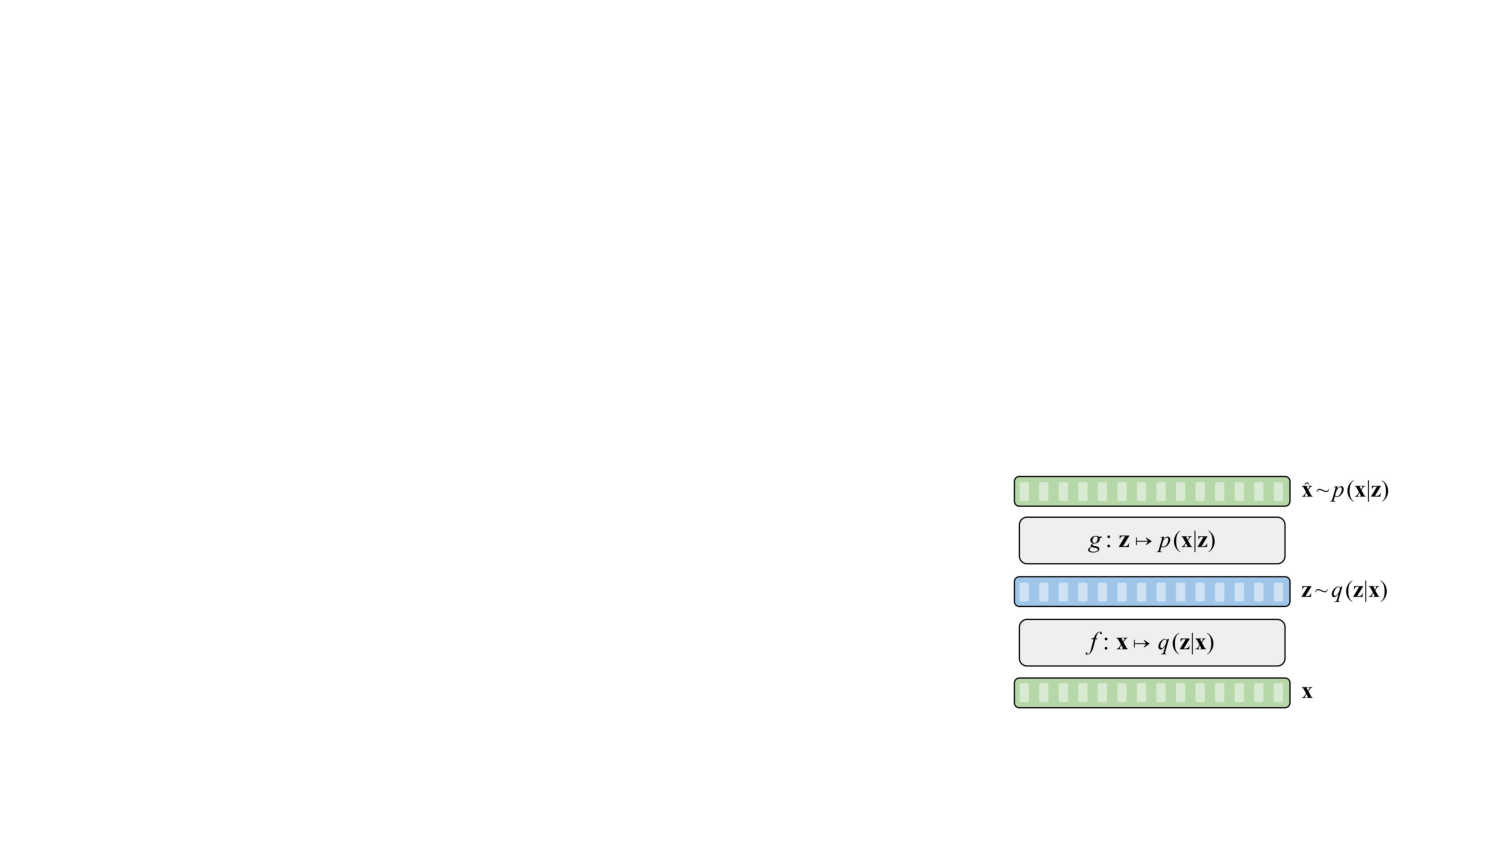
\includegraphics[height=0.4\textheight]{figures/brief-paradigms-lvm-2.pdf}};
                    \fill [draw=none, fill=white, fill opacity=0.7] (B.north west) -- (B.north east) -- (B.south east) -- (B.south west) -- (B.north west) -- cycle;
                }

                \only<2->{
                    \node[anchor=south west,inner sep=0] (A) at (0,0) {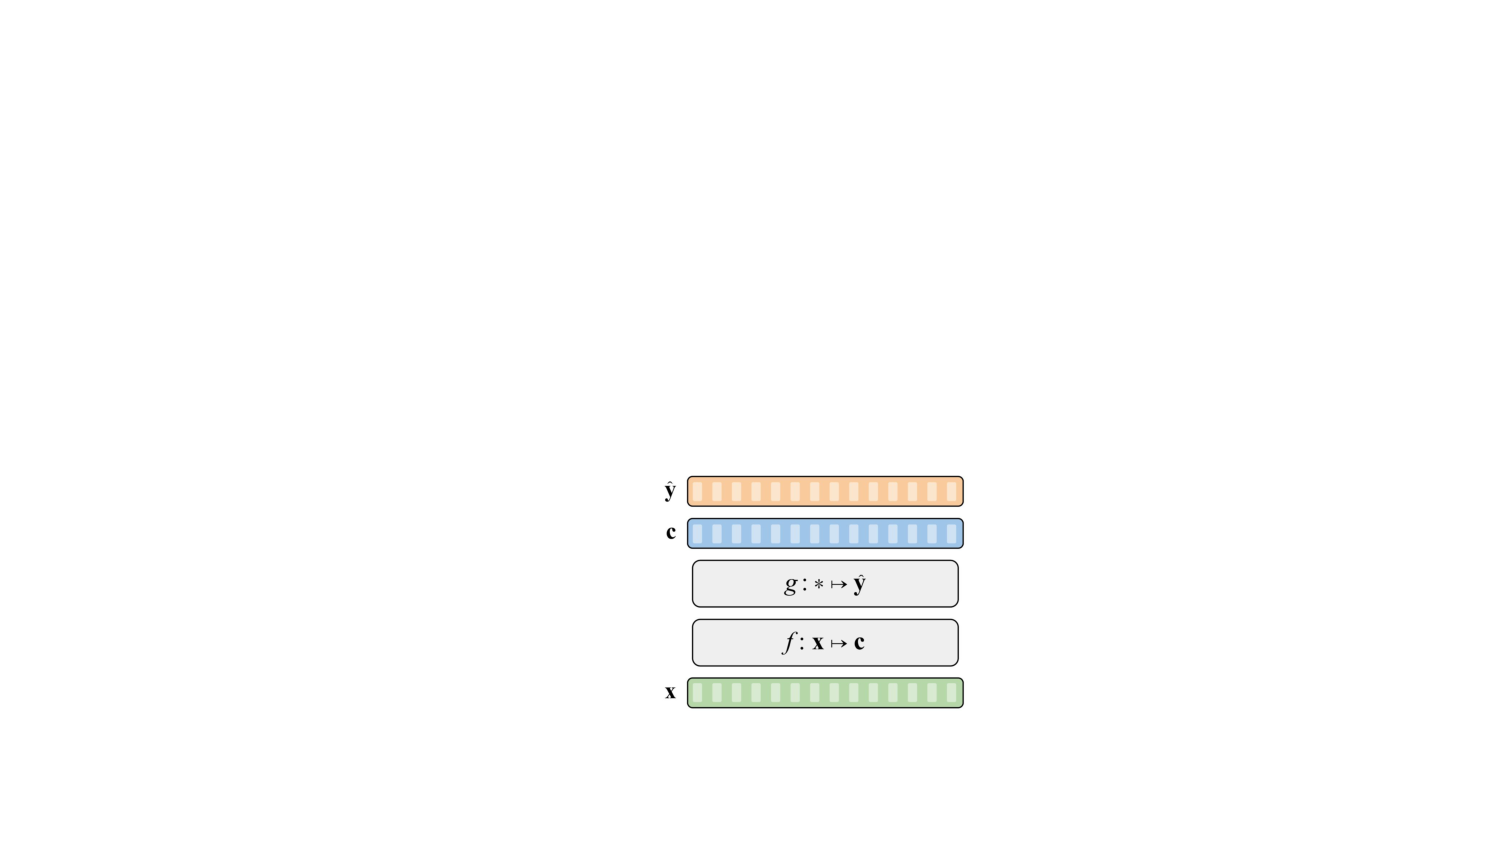
\includegraphics[height=0.4\textheight]{figures/brief-paradigms-ssl.pdf}};
                    \node[anchor=south west,inner sep=0] (B) at (4.2,0) {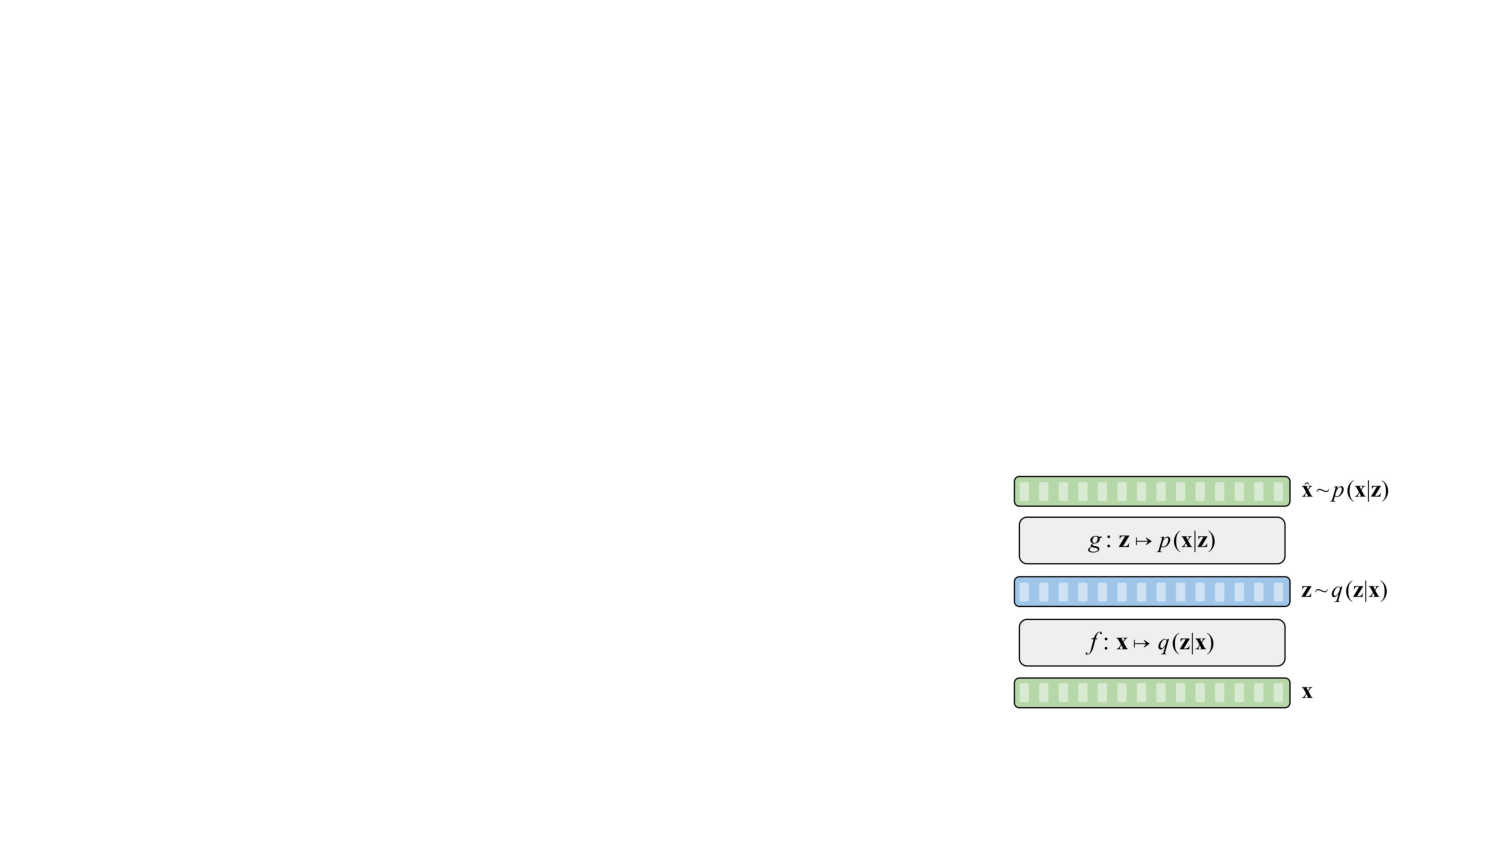
\includegraphics[height=0.4\textheight]{figures/brief-paradigms-lvm-2.pdf}};
                    \fill [draw=none, fill=white, fill opacity=0.7] (A.north west) -- (A.north east) -- (A.south east) -- (A.south west) -- (A.north west) -- cycle;
                }
            \end{tikzpicture}

        \end{column}
        
    \end{columns}
\end{frame}


\begin{frame}
    \frametitle{Graphical models for LVMs}
    % Figure TikZ sources at https://www.overleaf.com/project/61b212df9f315b5aec2b4a33
    \begin{columns}

        \begin{column}{0.5\textwidth}
            \begin{figure}
                \centering
                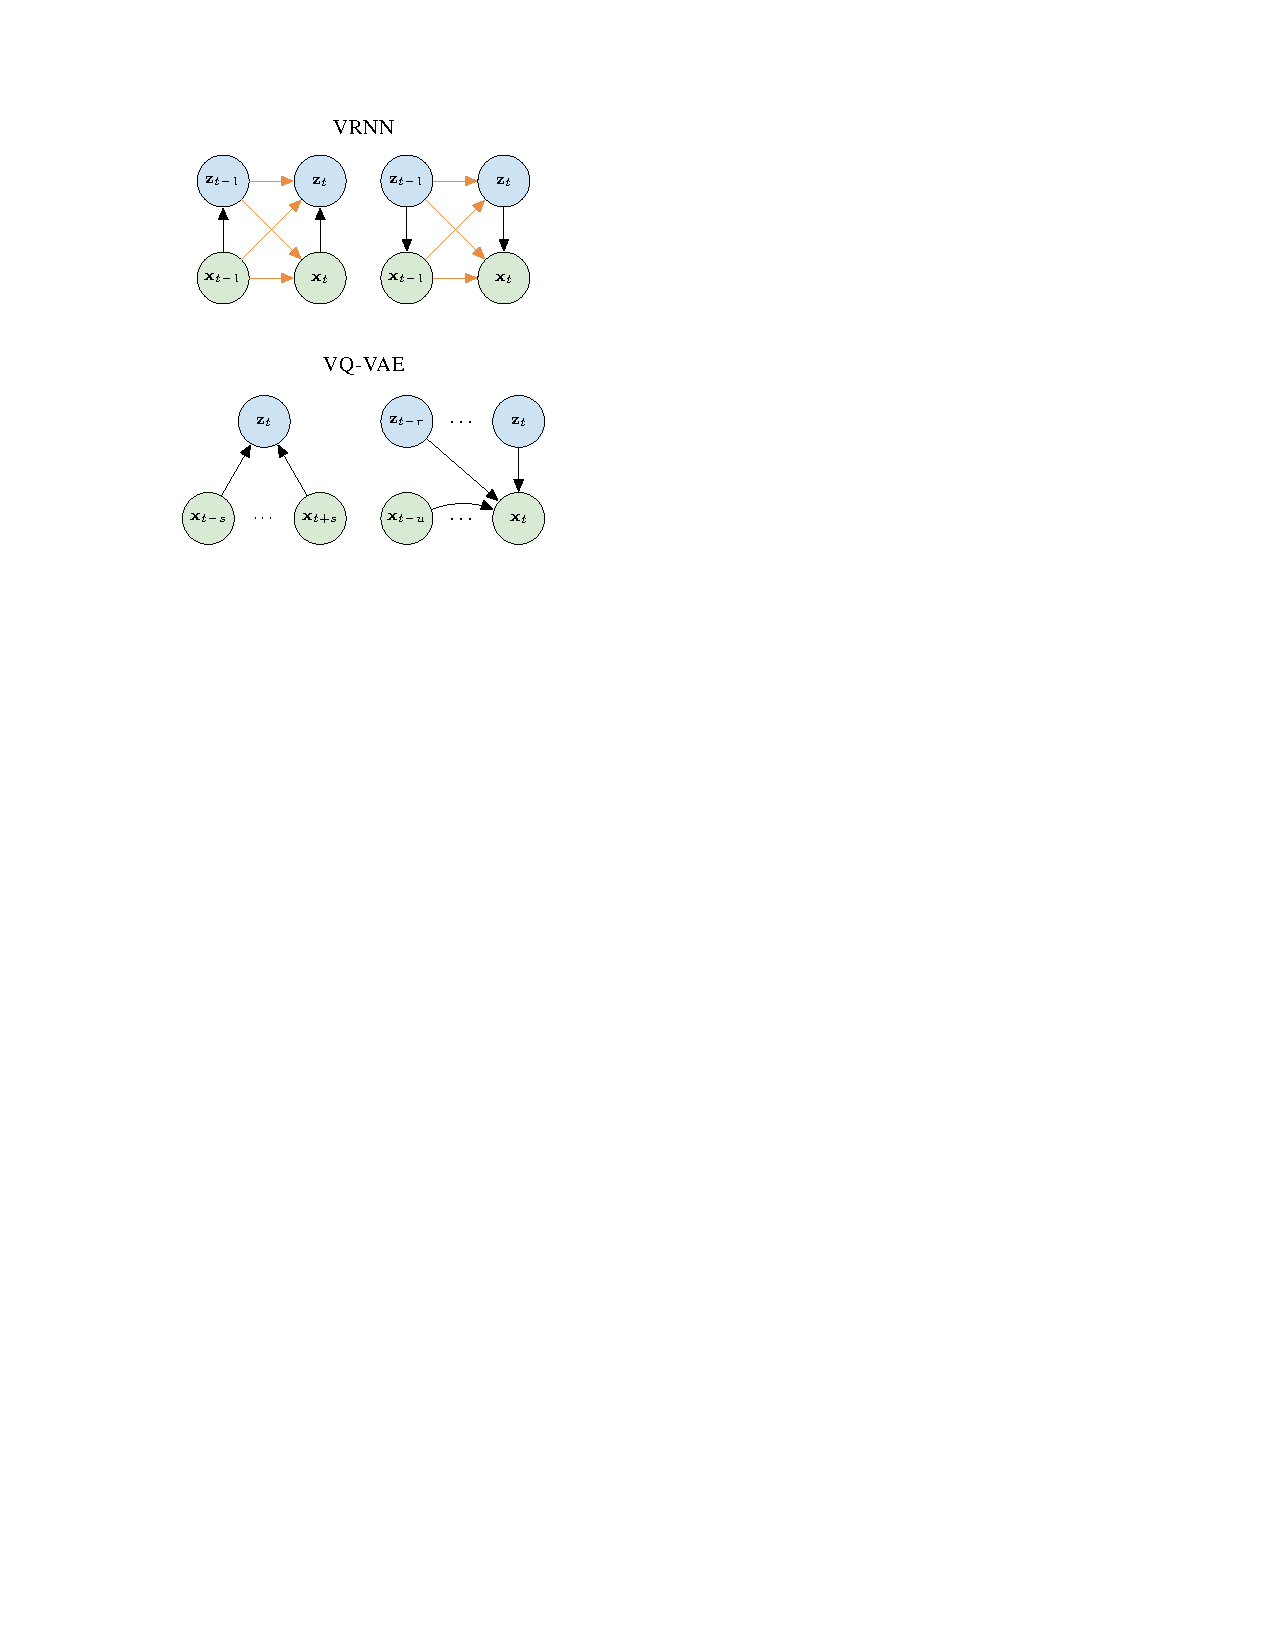
\includegraphics[width=0.8\textwidth]{figures/brief-vrnn-vqvae.pdf}
            \end{figure}
        \end{column}

        \begin{column}{0.5\textwidth}
            \begin{figure}
                \centering
                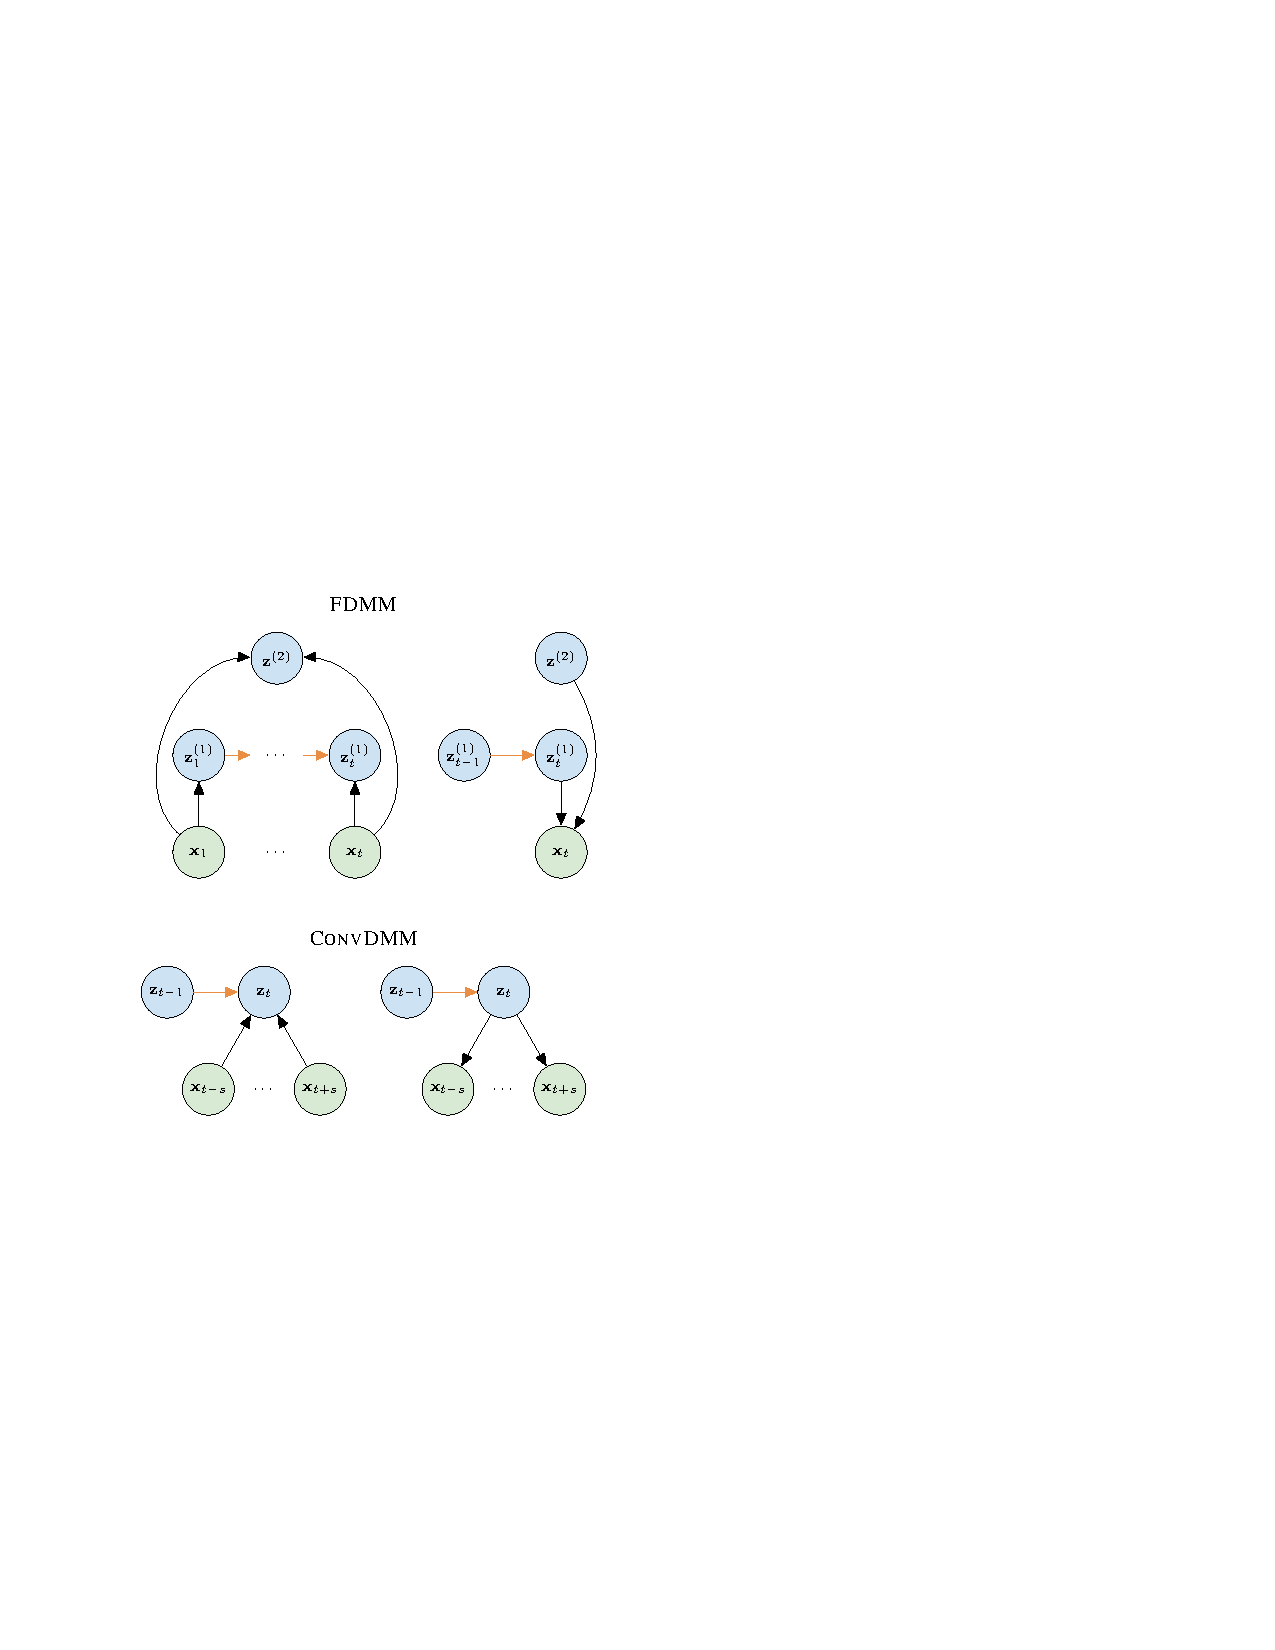
\includegraphics[width=0.8\textwidth]{figures/brief-fdmm-convdmm.pdf}
            \end{figure}            
        \end{column}

    \end{columns}

    \definecolor{sharedcolor}{RGB}{234 142 67} % mørk orange
    \blfootnote{\scalebox{0.6}{{\color{sharedcolor} Orange edges} indicate parameters shared between inference and generative models.}}
\end{frame}


\begin{frame}
    \frametitle{Overview of LVM probabilistic components}

    \begin{table}
        % \caption[A comprehensive overview of observation, prior and inference models for VAE type latent variable models with a single latent variable.]{ A comprehensive overview of observation, prior and inference models for VAE type latent variable models with a single latent variable. The observation, prior and inference models may all belong to one or more of the categories listed under them as detailed in \cref{sec:plvms}. The types listed here serve as primitives from which more complex structures can be constructed including models with hierarchies of multiple latent variables.}
        % \label{tab:lvm-model-primitives}
        % \begin{center}
        \centering
        % \renewcommand{\arraystretch}{1.1}
        \resizebox{0.8\textheight}{!}{%
            \begin{tabular}{ l l l } 
                \toprule
                \multicolumn{2}{l}{\textbf{\textsc{Type}}} & \textbf{\textsc{Form}} \\
                \midrule
                \multicolumn{3}{c}{\textsc{Observation model}} \\
                \midrule
                \textbf{\textsc{arx}} & Autoregressive on $\mathbf{x}_t$      & $p(\mathbf{x}_t|\mathbf{x}_{1:t-1})$ \\
                \textbf{\textsc{loc}} & Local latent variable                 & $p(\mathbf{x}_{t}|\mathbf{z}_{1:t})$ \\
                \textbf{\textsc{glb}} & Global latent variable                & $p(\mathbf{x}_{t}|\mathbf{z})$ \\
                \midrule
                \multicolumn{3}{c}{\textsc{Prior}} \\
                \midrule
                \textbf{\textsc{arx}} & Autoregressive on $\mathbf{x}_t$      & $p(\mathbf{z}_t|\mathbf{x}_{1:t-1})$ \\
                \textbf{\textsc{arz}} & Autoregressive on $\mathbf{z}_t$      & $p(\mathbf{z}_t|\mathbf{z}_{1:t-1})$ \\
                \textbf{\textsc{ind}} & Locally independent $\mathbf{z}_t$                 & $p(\mathbf{z}_t)$ \\
                \textbf{\textsc{glb}} & Global latent variable                & $p(\mathbf{z})$ \\
                \midrule
                \multicolumn{3}{c}{\textsc{Inference model}} \\
                \midrule
                \textbf{\textsc{arz}} & Autoregressive on $\mathbf{z}_t$      & $q(\mathbf{z}_t|\mathbf{z}_{1:t-1})$ \\
                \textbf{\textsc{flt}} & Filtering                             & $q(\mathbf{z}_t|\mathbf{x}_{1:t})$ \\
                \textbf{\textsc{lsm}} & Local smoothing                       & $q(\mathbf{z}_t|\mathbf{x}_{t-r:t+r})$ \\
                \textbf{\textsc{gsm}} & Global smoothing                      & $q(\mathbf{z}_t|\mathbf{x}_{1:T})$ \\
                \textbf{\textsc{glb}} & Global latent variable                & $q(\mathbf{z}|\mathbf{x}_{1:T})$ \\
                \bottomrule
            \end{tabular}
        }
        % \end{center}
    \end{table}

\end{frame}


\begin{frame}
    \frametitle{Classification of selected LVMs for speech}

    \begin{table}
        % \caption[Classification of selected latent variable models.]{ Selected latent variable models classified according the attributes defined throughout \cref{sec:plvms}. See \cref{tab:lvm-model-primitives} for the probability distributions that correspond to each of the attribute short-hands. \textbf{\textsc{hie}} indicates a hierarchical representation.}
        % \label{tab:lvm-taxonomy}
        % \begin{center}
        \centering
        \setlength{\tabcolsep}{3pt}
        \renewcommand{\arraystretch}{1.1}
        \resizebox{0.7\textwidth}{!}{%
            \begin{tabular}{ l | c c c | c c c c | c c c c c | c } 
                \toprule
                \multicolumn{2}{c}{} & 
                \multicolumn{3}{c}{\textsc{Observation}} & 
                \multicolumn{4}{c}{\textsc{Prior}} & 
                \multicolumn{5}{c}{\textsc{Inference}} \\
                \textbf{\textsc{model}} & 
                \textbf{\textsc{arx}} & 
                \textbf{\textsc{loc}} & 
                \textbf{\textsc{glb}} &  
                \textbf{\textsc{arx}} & 
                \textbf{\textsc{arz}} & 
                \textbf{\textsc{ind}} & 
                \textbf{\textsc{glb}} &  
                \textbf{\textsc{arz}} & 
                \textbf{\textsc{flt}} & 
                \textbf{\textsc{lsm}} & 
                \textbf{\textsc{gsm}} & 
                \textbf{\textsc{glb}} &
                \textbf{\textsc{hie}} \\
                \midrule
                %                                                              OBSERVATION       |              PRIOR                |                  INFERENCE       
                %                                                         ARX      LOC      GLB      ARX      ARZ     IND      GLB      ARZ      FLT      LSM      GSM      GLB
                \textbf{VRNN} \footnotesize{\parencite{chung_recurrent_2015}}          & \cmark & \cmark & \xmark & \cmark & \cmark & \xmark & \xmark & \cmark & \cmark & \xmark & \xmark & \xmark & \xmark \\
                \textbf{SRNN} \footnotesize{\parencite{fraccaro_sequential_2016}}      & \cmark & \cmark & \xmark & \cmark & \cmark & \xmark & \xmark & \cmark & \xmark & \xmark & \cmark & \xmark & \xmark \\
                \textbf{HMM-VAE} \footnotesize{\parencite{ebbers_hidden_2017}}         & \xmark & \cmark & \xmark & \xmark & \cmark & \xmark & \xmark & \cmark & \cmark & \xmark & \xmark & \xmark & \cmark \\
                \textbf{ConvVAE} \footnotesize{\parencite{hsu_learning_2017}}          & \xmark & \xmark & \cmark & \xmark & \xmark & \xmark & \cmark & \xmark & \xmark & \xmark & \cmark & \cmark & \xmark \\
                \textbf{FHVAE} \footnotesize{\parencite{hsu_unsupervised_2017}}        & \xmark & \cmark & \cmark & \xmark & \xmark & \cmark & \cmark & \xmark & \xmark & \xmark & \cmark & \cmark & \cmark \\
                \textbf{VQ-VAE} \footnotesize{\parencite{oord_neural_2018}}            & \cmark & \cmark & \xmark & \xmark & \xmark & \cmark & \xmark & \xmark & \xmark & \cmark & \xmark & \xmark & \xmark \\
                \textbf{BHMM-VAE} \footnotesize{\parencite{glarner_full_2018}}         & \xmark & \cmark & \xmark & \xmark & \cmark & \xmark & \xmark & \cmark & \cmark & \xmark & \xmark & \xmark & \xmark \\
                \textbf{STCN} \footnotesize{\parencite{aksan_stcn_2019}}               & \xmark & \cmark & \xmark & \cmark & \xmark & \xmark & \xmark & \xmark & \cmark & \xmark & \xmark & \xmark & \cmark \\
                \textbf{FDMM} \footnotesize{\parencite{khurana_factorial_2019}}        & \xmark & \cmark & \cmark & \xmark & \cmark & \xmark & \cmark & \cmark & \cmark & \xmark & \xmark & \cmark & \cmark \\
                \textbf{ConvDMM} \footnotesize{\parencite{khurana_convolutional_2020}} & \xmark & \cmark & \xmark & \xmark & \cmark & \xmark & \xmark & \cmark & \xmark & \cmark & \xmark & \xmark & \xmark \\
                \bottomrule
            \end{tabular}
        }
        % \end{center}
    \end{table}

\end{frame}

\begin{frame}
    \frametitle{Comparison of LVMs and SSL methods}

    \begin{table}
        % \caption[Classification of selected self"=supervised and probabilistic latent variable models.]{ Selected models classified according to the binary attributes identified throughout the text. The models are sorted according to first publication date on arXiv which might differ from the citation year. \textbf{\textsc{msk}}: masking, \textbf{\textsc{prd}}: prediction, \textbf{\textsc{con}}: contrastive, \textbf{\textsc{rec}}: reconstruction, \textbf{\textsc{qtz}}: quantization, \textbf{\textsc{gen}}: generative, \textbf{\textsc{frz}}: frozen, \textbf{\textsc{ftn}}: fine"=tuned, \textbf{\textsc{loc}}: local, \textbf{\textsc{glo}}: global.}
        % \label{tab:model-taxonomy}
        % \begin{center}
        \centering
        \setlength{\tabcolsep}{3pt}
        \renewcommand{\arraystretch}{1.1}
        \resizebox{1\textheight}{!}{%
            \begin{tabular}{ l l | c c c c c c | c c c | c c } 
                \toprule
                
                \multicolumn{2}{c}{} & 
                \multicolumn{6}{c}{\textsc{model and task design}} & 
                \multicolumn{3}{c}{\textsc{resolution}} &
                \multicolumn{2}{c}{\makebox[0pt][c]{\textsc{usage}}} \\
                & \textbf{\textsc{model}} &
                \textbf{\textsc{msk}} & 
                \textbf{\textsc{prd}} & 
                \textbf{\textsc{con}} &  
                \textbf{\textsc{rec}} &  
                \textbf{\textsc{qtz}} & 
                \textbf{\textsc{gen}} & 
                \textbf{\textsc{loc}} & 
                \textbf{\textsc{glb}} & 
                \textbf{\textsc{var}} & 
                \textbf{\textsc{frz}} & 
                \textbf{\textsc{ftn}} \\
                
                \midrule
                % \multicolumn{11}{c}{\textsc{Self-supervised models}} \\
                % \midrule
                %                                                           MSK      PRD      CON      REC      QTZ      GEN      LOC      GLB     VAR      FRZ      FTN
                \verticalmultirow{9}{\textsc{Self-supervised models}} 
                % & \textbf{Audio Word2vec} \footnotesize{\parencite{chung_audio_2016}}      & \cmark & \xmark & \xmark & \cmark & \xmark & \xmark & \xmark & \cmark & \xmark & \cmark & \xmark \\
                % & \textbf{Speech2Vec} \footnotesize{\parencite{chung_speech2vec_2018}}     & \xmark & \cmark & \xmark & \cmark & \xmark & \xmark & \xmark & \cmark & \xmark & \cmark & \xmark \\
                % & \textbf{Unspeech} \footnotesize{\parencite{milde_unspeech_2018}}         & \xmark & \cmark & \cmark & \xmark & \xmark & \xmark & \xmark & \cmark & \xmark & \cmark & \xmark \\
                
                & \textbf{CPC} \footnotesize{\parencite{oord_representation_2018}}         & \xmark & \cmark & \cmark & \xmark & \xmark & \xmark & \cmark & \xmark & \xmark & \cmark & \xmark \\
                
                & \textbf{APC} \footnotesize{\parencite{chung_unsupervised_2019}}          & \xmark & \cmark & \xmark & \cmark & \xmark & \xmark & \cmark & \xmark & \xmark & \cmark & \xmark \\ % 5/4
                & \textbf{wav2vec} \footnotesize{\parencite{schneider_wav2vec_2019}}       & \xmark & \cmark & \cmark & \xmark & \xmark & \xmark & \cmark & \xmark & \xmark & \cmark & \xmark \\ % 11/4
                & \textbf{Mockingjay}  \footnotesize{\parencite{liu_mockingjay_2020}}      & \cmark & \xmark & \xmark & \cmark & \xmark & \xmark & \cmark & \xmark & \xmark & \cmark & \cmark \\ % 25/10-19
                & \textbf{wav2vec 2.0} \footnotesize{\parencite{baevski_wav2vec_2020}}     & \cmark & \xmark & \cmark & \xmark & \cmark & \xmark & \cmark & \xmark & \xmark & \xmark & \cmark \\ % 20/6
                & \textbf{NPC} \footnotesize{\parencite{liu_nonautoregressive_2020}}       & \cmark & \xmark & \xmark & \cmark & \cmark & \xmark & \cmark & \xmark & \xmark & \cmark & \xmark \\ % 1/11
                & \textbf{DeCoAR 2.0} \footnotesize{\parencite{ling_decoar_2020}}          & \cmark & \xmark & \xmark & \cmark & \cmark & \xmark & \cmark & \xmark & \xmark & \cmark & \xmark \\ % 11/12
                % & \textbf{SCPC} \footnotesize{\parencite{bhati_segmental_2021}}            & \xmark & \cmark & \cmark & \xmark & \xmark & \xmark & \cmark & \xmark & \cmark & \cmark & \xmark \\ % 3/6
                & \textbf{HuBERT} \footnotesize{\parencite{hsu_hubert_2021}}               & \cmark & \xmark & \xmark & \xmark & \cmark & \xmark & \cmark & \xmark & \xmark & \xmark & \cmark \\ % 14/6
                & \textbf{data2vec} \footnotesize{\parencite{baevski_data2vec_2022}}       & \cmark & \xmark & \xmark & \xmark & \xmark & \xmark & \cmark & \xmark & \xmark & \xmark & \cmark \\ % 16/6

                \midrule
                % \multicolumn{11}{c}{\textsc{Probabilistic latent variable models}} \\
                % \midrule
                %                                                           MSK      PRD      CON      REC      QTZ      GEN      LOC      GLO     VAR      FRZ      FTN
                \verticalmultirow{8}{\textsc{Latent variable models}}
                & \textbf{VRNN} \footnotesize{\parencite{chung_recurrent_2015}}          & \xmark & \xmark & \xmark & \cmark & \xmark & \cmark & \cmark & \xmark & \xmark & \cmark & \xmark \\
                & \textbf{SRNN} \footnotesize{\parencite{fraccaro_sequential_2016}}      &\xmark & \xmark & \xmark & \cmark & \xmark & \cmark & \cmark & \xmark & \xmark & \cmark & \xmark \\
                % & \textbf{HMM-VAE} \footnotesize{\parencite{ebbers_hidden_2017}}         & \xmark & \xmark & \xmark & \cmark & \xmark & \cmark & \cmark & \xmark & \xmark & \cmark & \xmark \\
                & \textbf{ConvVAE} \footnotesize{\parencite{hsu_learning_2017}}          & \xmark & \xmark & \xmark & \cmark & \xmark & \cmark & \xmark & \cmark & \xmark & \cmark & \xmark \\
                & \textbf{FHVAE} \footnotesize{\parencite{hsu_unsupervised_2017}}        & \xmark & \xmark & \xmark & \cmark & \xmark & \cmark & \cmark & \cmark & \xmark & \cmark & \xmark \\
                & \textbf{VQ-VAE} \footnotesize{\parencite{oord_neural_2018}}            & \xmark & \xmark & \xmark & \cmark & \cmark & \cmark & \cmark & \xmark & \xmark & \cmark & \xmark \\
                % & \textbf{BHMM-VAE} \footnotesize{\parencite{glarner_full_2018}}         & \xmark & \xmark & \xmark & \cmark & \xmark & \cmark & \cmark & \xmark & \xmark & \cmark & \xmark \\
                & \textbf{STCN} \footnotesize{\parencite{aksan_stcn_2019}}               & \xmark & \xmark & \xmark & \cmark & \xmark & \cmark & \cmark & \xmark & \xmark & \cmark & \xmark \\
                & \textbf{FDMM} \footnotesize{\parencite{khurana_factorial_2019}}        & \xmark & \xmark & \xmark & \cmark & \xmark & \cmark & \cmark & \cmark & \xmark & \cmark & \xmark \\
                & \textbf{ConvDMM} \footnotesize{\parencite{khurana_convolutional_2020}} & \xmark & \xmark & \xmark & \cmark & \xmark & \cmark & \cmark & \xmark & \xmark & \cmark & \xmark \\
                \bottomrule
            \end{tabular}
        }
        % \end{center}
    \end{table}

\end{frame}


% ======================================================================================================================


